% CE7454 Assignment 1 report, built on the CVPR 2026 author kit
% (https://github.com/cvpr-org/author-kit). Compile with pdflatex + bibtex.

\documentclass[10pt,twocolumn,letterpaper]{article}

%%%%%%%%% PAPER TYPE
% \usepackage[review]{cvpr}      % review version (line numbers, anonymous)
\usepackage[pagenumbers]{cvpr}   % camera-ready layout with page numbers

%% This file contains a number of tweaks that are typically applied to the main document.
%% They are not enabled by default, but can be enabled by uncommenting the relevant lines.


%%
%% Official support for 2-column teaser figure
%%
\usepackage{cuted} %< for strip environment

%%
%% For auto-referencing of figures (see fig/teaser.tex and \label{} therein) 
%%
\usepackage{currfile} %< for \currfilebase macro

%%
%% caption and (global) spacing overrides
%%
\usepackage{caption} %< for "\captionof" commands (teaser)
% \setlength{\abovecaptionskip}{.5em} % space above caption
% \setlength{\belowcaptionskip}{1em} % space below caption

%%
%% Inline annotations; for predefined colors, refer to "dvipsnames" in the xcolor package:
%% https://tinyurl.com/overleaf-colors
%%
\newcommand{\red}[1]{{\color{red}#1}}
\newcommand{\todo}[1]{{\color{red}#1}}
\newcommand{\TODO}[1]{\textbf{\color{red}[TODO: #1]}}
%%
%% Disable for camera ready / submission by uncommenting these lines:
%%
% \renewcommand{\TODO}[1]{}
% \renewcommand{\todo}[1]{#1}

%%
%% Work harder in optimizing text layout. Typically shrinks text by 1/6 of page, enable
%% it at the very end of the writing process, when you are just above the page limit.
%%
\usepackage{microtype}

%%
%% Fine-tune paragraph spacing.
%%
% \renewcommand{\paragraph}[1]{\vspace{.5em}\noindent\textbf{#1.}}

%%
%% Globally adjusts space between figure and caption.
%%
% \setlength{\abovecaptionskip}{.5em}

%%
%% Allows "the use of \paper to refer to the project name"
%% with automatic management of space at the end of the word.
%%
% \usepackage{xspace}
% \newcommand{\paper}{ProjectName\xspace}

%%
%% Commonly used math definitions.
%%
% \DeclareMathOperator*{\argmin}{arg\,min}
% \DeclareMathOperator*{\argmax}{arg\,max}

%%
%% Tighten underline.
%%
% \usepackage{soul}
% \setuldepth{foobar}

%%
%% Reconfigure paragraph (tweaks spacing)
%%

\usepackage{tikz}
\usetikzlibrary{arrows.meta,positioning,fit,calc}

\definecolor{cvprblue}{rgb}{0.21,0.49,0.74}
\usepackage[pagebackref,breaklinks,colorlinks,allcolors=cvprblue]{hyperref}

\def\paperID{CE7454}
\def\confName{CVPR}
\def\confYear{2026}

\title{A Perfect Detector Undone by a 0.8\% Rescale:\\
Phase-Robust Three-Way Generator Attribution from Scratch}

\author{Pugalia Aditya Kumar\\
Graduate College (IGP AI-X), Nanyang Technological University\\
{\tt\small Adityaku004@e.ntu.edu.sg}
}

\begin{document}
\maketitle
\begin{abstract}
We attribute $512\times512$ JPEGs to a camera or to one of two undisclosed generators with a single from-scratch model of at most 12.3M parameters. A ResNet-18 that reads the image and its neighbouring-pixel residual at full resolution scores 100\% on held-out and development data, yet labels all 1,500 test images as real. From the unlabelled test spectra we infer why: the test images were stretched by about $512/508$ and re-encoded as JPEG q90 4:2:0. The stretch shifts the generators' period-8 up-sampling lattice by up to 4 pixels, and the detector is locked to that lattice's phase. Our submitted model, v4, keeps the residual input but down-samples with anti-aliasing BlurPool layers. It is trained on $256^2$ crops of 152k stored, broadly augmented copies and applied once to each test image as given. It scores \textbf{95.3\%} on test (the baseline's all-real output scores 33.3\%) and 96.1\% on development data. Probes show that v4 is invariant to sub-period shifts and flips. An ablation shows that augmentation narrowly matched to the inferred processing overfits it. Almost all remaining errors are real photographs labelled as fake.
\end{abstract}

\section{Introduction}
\label{sec:intro}

The project is based on an AI generated image detection task where the pipeline needs to distinguish between a real image (class~0) or one of two undisclosed generators, Model~A (class 1) and Model~B (class 2). The training data had 15,000 labelled $512\times512$ JPEGs with equal distribution for each class. For this task a model using ResNet style architecture with about 11.17M trainable parameters was trained from scratch using no external data, ensembles, distillation or test-time methods.

Image generators create images by repeatedly up-sampling a small feature map to full resolution, usually with transposed convolutions or nearest-neighbour interpolation followed by convolution. Each output pixel is computed from a few input values, and neighbouring pixels are therefore correlated in a fixed, periodic way ~\cite{odena2016checkerboard,zhang2019spectrum,tan2024npr}. A small ResNet that is given these correlations explicitly, through the neighbouring-pixel residual (NPR)~\cite{tan2024npr} and a stem without stride~\cite{gragnaniello2021critical}, scores 100\% on the validation set and dev data. However, on the test set it labels \emph{every} image as real. The test images had been post-processed, showing that even though the simple ResNet architecture can accurately learn the generators' pattern, it is not invariant to transformations.

\noindent\textbf{Contributions.}
An augmentation-robust detector that combines BlurPool down-sampling~\cite{zhang2019blurpool}, crop training and broad offline augmentation to accurately classify the image source.

\section{Related Work}
\label{sec:related}
\noindent\textbf{Generator artifacts.} Most image generators build an image by up-sampling a low-resolution feature map several times. Odena \etal~\cite{odena2016checkerboard} showed that a transposed convolution whose kernel size is not divisible by its stride covers some output pixels more often than others, which produces a visible checkerboard pattern. Even when the pattern is not visible, it remains in the frequency domain. Up-sampling repeats the spectrum of the low-resolution map, so generated images have periodic peaks in their Fourier or DCT spectra that real photographs lack, and a simple classifier on the spectrum detects them reliably~\cite{zhang2019spectrum,frank2020frequency}. Each trained model leaves its own fingerprint in the noise residual of its images, which is enough to tell apart models with the same architecture~\cite{yu2019attribution,marra2019fingerprints}. That is the property our three-way task relies on. Tan \etal~\cite{tan2024npr} exploit the up-sampling directly with the neighbouring-pixel residual (NPR). Nearest-neighbour up-sampling copies one value into a $2\times2$ block, so subtracting each pixel from its neighbour in the block removes image content and leaves the up-sampling trace. This is used as an input to our network.

\noindent\textbf{Robust detection.} A detector that works on clean images can still fail once the images are post-processed. Wang \etal~\cite{wang2020cnndetect} trained a ResNet-50 on a single GAN and found that random blur and JPEG compression during training were what let it generalise to unseen generators and to compressed images. Gragnaniello \etal~\cite{gragnaniello2021critical} showed that the network's early layers matter as much. Strided convolutions and pooling at the start of a standard ResNet throw away the high-frequency detail that carries the artifacts, so removing that early down-sampling and training on unresized crops gives a large gain, a recipe Corvi \etal~\cite{corvi2023diffusion} also adopt for diffusion images. Chai \etal~\cite{chai2020patch} found that classifiers with a small receptive field, which judge each patch separately, generalise better than whole-image classifiers. This suggests the evidence is local and repeated across the image. The same down-sampling also makes CNNs sensitive to small shifts. Because a strided layer samples its input without first low-pass filtering it, moving the image by a single pixel can change the prediction~\cite{azulay2019small}. BlurPool~\cite{zhang2019blurpool} fixes this by blurring before each down-sampling step. Popescu and Farid~\cite{popescu2005resampling} showed that rescaling an image introduces periodic correlations between neighbouring pixels, the same kind of signal that up-sampling generators leave. 

\section{Method}
\label{sec:method}

% Fig. 1: training-data pipeline (top) and network (bottom). Pure TikZ, compiles on Overleaf.
\begin{figure*}[t]
\centering
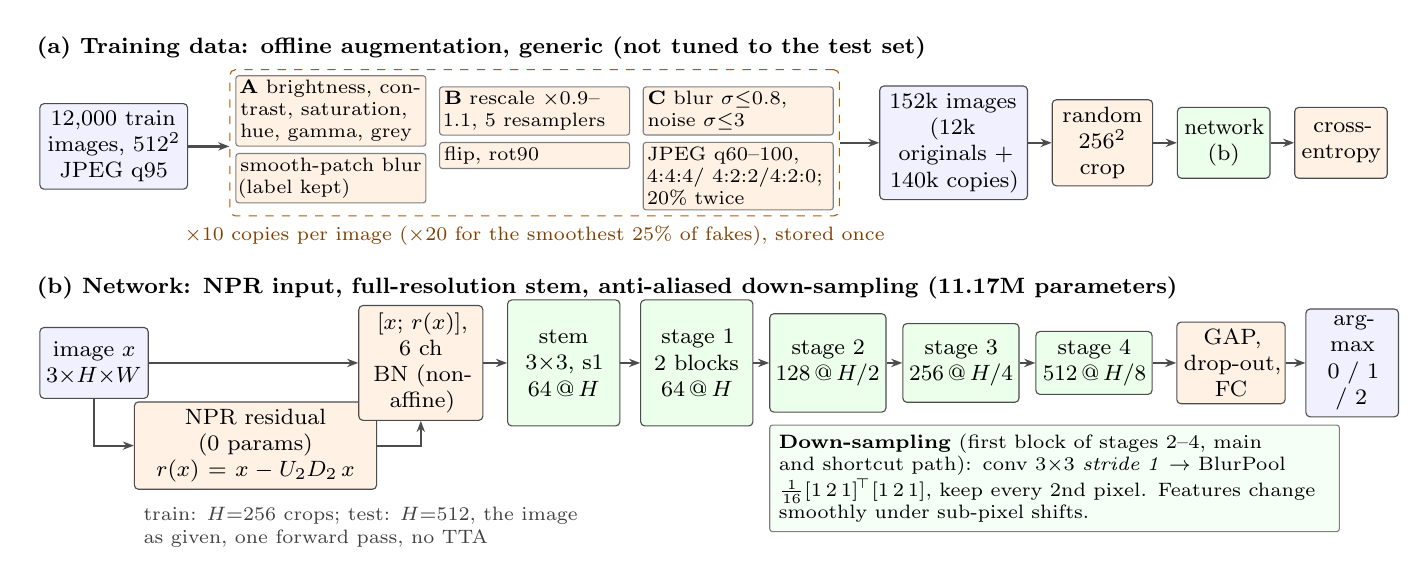
\begin{tikzpicture}[
    font=\footnotesize, >={Stealth[length=4pt]}, node distance=3mm,
    box/.style={draw=black!70, rounded corners=1.5pt, align=center, inner sep=2.5pt, minimum height=9mm},
    data/.style={box, fill=blue!6},
    op/.style={box, fill=orange!10},
    aug/.style={draw=black!50, rounded corners=1pt, fill=orange!10, align=left, inner sep=1.6pt, font=\scriptsize, text width=23mm},
    net/.style={box, fill=green!8},
    lab/.style={font=\footnotesize\bfseries, anchor=west},
    arr/.style={->, thick, black!70}]
% ---------------------------------------------------------------- (a) data
\node[lab] at (-0.55, 1.25) {(a) Training data: offline augmentation, generic (not tuned to the test set)};
\node[data, text width=17mm] (src) at (0.55,0) {12,000 train\\images, $512^2$\\JPEG q95};
\node[aug, right=6mm of src, yshift=4.5mm] (a1) {\textbf{A} brightness, contrast, saturation, hue, gamma, grey};
\node[aug, below=0.8mm of a1] (a2) {smooth-patch blur (label kept)};
\node[aug, right=1.6mm of a1] (b1) {\textbf{B} rescale $\times$0.9--1.1, 5 resamplers};
\node[aug, below=0.8mm of b1] (b2) {flip, rot90};
\node[aug, right=1.6mm of b1] (c1) {\textbf{C} blur $\sigma{\le}0.8$, noise $\sigma{\le}3$};
\node[aug, below=0.8mm of c1] (c2) {JPEG q60--100, 4:4:4/ 4:2:2/4:2:0; 20\% twice};
\node[draw=orange!70!black, dashed, rounded corners=2pt, inner sep=2pt, fit=(a1)(a2)(b1)(b2)(c1)(c2),
      label={[font=\scriptsize, text=orange!50!black]below:$\times10$ copies per image ($\times20$ for the smoothest 25\% of fakes), stored once}] (augbox) {};
\node[data, right=5mm of augbox, text width=17mm] (store) {152k images\\(12k originals +\\140k copies)};
\node[op, right=of store, text width=11mm] (crop) {random\\$256^2$ crop};
\node[net, right=of crop, text width=10mm] (netA) {network\\(b)};
\node[op, right=of netA, text width=10mm] (ce) {cross-\\entropy};
\draw[arr] (src) -- (src -| augbox.west);
\draw[arr] (augbox) -- (store); \draw[arr] (store) -- (crop); \draw[arr] (crop) -- (netA); \draw[arr] (netA) -- (ce);
% ---------------------------------------------------------------- (b) network
\begin{scope}[yshift=-2.75cm]
\node[lab] at (-0.55, 0.95) {(b) Network: NPR input, full-resolution stem, anti-aliased down-sampling (11.17M parameters)};
\node[data, text width=12mm] (x) at (0.3,0) {image $x$\\$3{\times}H{\times}W$};
\node[op, text width=29mm, minimum height=6mm] (npr) at (2.35,-1.05) {NPR residual (0 params)\\$r(x)=x-U_2D_2\,x$};
\node[op, text width=14mm] (cat) at (4.45,0) {$[x;\,r(x)]$, 6 ch\\BN (non-affine)};
\draw[arr] (x) -- (cat); \draw[arr] (x.south) |- (npr.west); \draw[arr] (npr.east) -| (cat.south);
\node[net, right=3mm of cat, text width=12.5mm, minimum height=16mm] (stem) {stem\\$3{\times}3$, s1\\64\,@\,$H$};
\node[net, right=2.5mm of stem, text width=12.5mm, minimum height=16mm] (s1) {stage 1\\2 blocks\\64\,@\,$H$};
\node[net, right=2mm of s1, text width=13mm, minimum height=12.5mm] (s2) {stage 2\\128\,@\,$H/2$};
\node[net, right=2mm of s2, text width=13mm, minimum height=10mm] (s3) {stage 3\\256\,@\,$H/4$};
\node[net, right=2mm of s3, text width=13mm, minimum height=8mm] (s4) {stage 4\\512\,@\,$H/8$};
\node[op, right=3mm of s4, text width=12mm] (head) {GAP, drop-out, FC};
\node[data, right=2.5mm of head, text width=10mm] (out) {arg-max\\0 / 1 / 2};
\foreach \a/\b in {cat/stem, stem/s1, s1/s2, s2/s3, s3/s4, s4/head, head/out} \draw[arr] (\a) -- (\b);
\node[draw=black!50, rounded corners=1pt, fill=green!4, align=left, font=\scriptsize, text width=70mm, anchor=north west] (bp)
  at ($(s2.south west)+(0,-1.5mm)$)
  {\textbf{Down-sampling} (first block of stages 2--4, main and shortcut path): conv $3{\times}3$ \emph{stride 1} $\to$ BlurPool $\frac{1}{16}[1\,2\,1]^{\!\top}[1\,2\,1]$, keep every 2nd pixel. Features change smoothly under sub-pixel shifts.};
\node[font=\scriptsize, align=left, text=black!75, anchor=north west] at ($(npr.south west)+(0,-1mm)$)
  {train: $H{=}256$ crops; test: $H{=}512$, the image\\as given, one forward pass, no TTA};
\end{scope}
\end{tikzpicture}
\vspace{-1mm}
\caption{\textbf{Overview.} (a) Each training image is turned into 10 (or 20) stored augmented copies whose operations bracket, but are not fitted to, the unknown test-time processing; training draws a random $256^2$ crop. (b) The fully convolutional ArtifactResNet reads the RGB image and its neighbouring-pixel residual at full resolution and down-samples only through blurred (anti-aliased) strides, so it can be trained on crops and applied to whole $512^2$ test images.}
\label{fig:overview}
\vspace{-2mm}
\end{figure*}


\subsection{Exploratory analysis}
\label{sec:eda}
The training classes are balanced (5,000 each), and every image is a $512^2$ JPEG at quality~95 with 4:4:4 chroma. To look for up-sampling traces, we averaged the log-magnitude Fourier spectrum of the image minus its $3\times3$ binomial blur over 200 images per class. A pattern that repeats every $p$ pixels gives a peak at bin $512/p$ in the Fourier transformation. All classes, real photographs included, have peaks on the axes at bins 64, 128 and 256, which come from the $8\times8$ block grid of JPEG. Both generators therefore leave a 2-D grid with periods of 2, 4 and 8 pixels, consistent with repeated $2\times$ up-sampling~\cite{odena2016checkerboard,zhang2019spectrum}, and it is stronger for Model~B. Thus, the input should expose the correlations between neighbouring pixels.

\subsection{Setting and baseline}
\label{sec:baseline}

\noindent\textbf{Residual input.} Let $x \in \mathbb{R}^{3\times H\times W}$ be the input RGB image. We define two fixed operators. The down-sampling operator $D_2$ keeps only the top-left pixel of every non-overlapping $2\times2$ block, giving an image of size $\frac{H}{2}\times\frac{W}{2}$. The up-sampling operator $U_2$ is nearest-neighbour up-sampling by two, which copies each pixel back into a $2\times2$ block. Applying both, $U_2 D_2\, x$, therefore gives an $H\times W$ image in which every pixel is replaced by the top-left pixel of its block. The neighbouring-pixel residual (NPR)~\cite{tan2024npr} is the difference between the image and this copy,
\begin{equation}
  r(x) = x - U_2 D_2\, x
  \label{eq:npr}
\end{equation}
  $r$ removes most of the image content and remains are the correlations between adjacent pixels that generator up-sampling layers introduce. The network receives the six-channel concatenation $[x;\,r(x)]$. Because $|r|$ is about 20 times smaller than $|x|$, both are first normalised by a BatchNorm layer with no learnable scale or shift which puts the two inputs on a similar scale without adding parameters.


\noindent\textbf{Baseline.} A ResNet-18~\cite{he2016resnet} with a $3\times3$, stride-1 stem and no max-pool, so stage~1 sees every residual pixel~\cite{gragnaniello2021critical}. It ends with global average pooling, dropout 0.2 and a linear layer (\cref{fig:overview}b). The \emph{baseline} is trained on whole $512^2$ images without augmentation and with early-stopping (AdamW, lr $10^{-3}$).

\subsection{Diagnosing the test shift}
\label{sec:diagnosis}
The unlabelled test images differ from the training images in two ways. The generators' repeating pattern sits at a different position and spacing in their spectra (\cref{fig:diagnosis}), and the images are more strongly compressed. Their content may also come from a different distribution from what the training data is used to. As a result, the baseline which was trained on plain training data predicted all images as real on the test set as it was not invariant to transformations.


\begin{figure}[t]
  \centering
  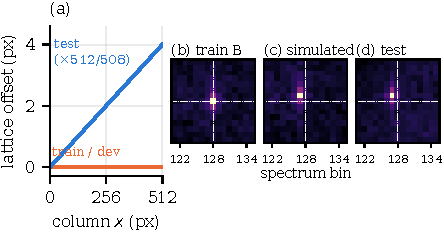
\includegraphics[width=\linewidth]{fig/diagnosis.pdf}
  \caption{\textbf{Diagnosis.} (a) Offset of the generators' 8-pixel lattice relative to the image origin along a row. It is constant in training and dev images and drifts by up to 4~px in test images after a $512/508$ stretch. (b--d) Mean log-magnitude spectrum of the high-pass luma around the period-4 diagonal site at bin 128 (dotted lines). The peak sits exactly at 128 for Model~B training images (b) and moves to 127 after our simulated processing (c), matching the real test set (d).}
  \label{fig:diagnosis}
\end{figure}

\subsection{A transformation-robust detector}
\label{sec:v4}
To make the Baseline ResNet model more robust to different distributions and transformations, the followiing changes to the architecture and training were applied:

\noindent\textbf{Anti-aliased down-sampling.} A stride-2 convolution keeps one pixel in four, so its output depends on the input position modulo 2. Stacked over three stages, the features depend on the position modulo 8, exactly the lattice period~\cite{azulay2019small}. In stages 2--4 we replace each stride-2 convolution, and its $1\times1$ shortcut, by a stride-1 convolution followed by BlurPool~\cite{zhang2019blurpool}:
\begin{equation}
  \mathrm{BP}(h) = \big(h * \tfrac{1}{16}[1\;2\;1]^{\top}[1\;2\;1]\big)\!\downarrow_2 .
\end{equation}
BlurPool has no parameters. NPR keeps its $2\times2$ anchoring, so full invariance must still be learnt from data.

\noindent\textbf{Offline augmentation.} We store 10 augmented copies of every training image, and 20 copies for the 25\% of fakes with the least texture (mean absolute luma high-pass), which are the hardest fakes. That gives 140k copies, plus the 12k originals (\cref{fig:overview}a). Each copy passes through a random chain:
(A)~brightness and contrast $\times$[0.8,\,1.2] ($p{=}.5$), saturation $\times$[0.5,\,1.3] (.5), hue $\pm$0.03 (.2), gamma [0.8,\,1.25] (.3), greyscale (.05), and blurring of 1--2 rectangles covering 10--40\% of the image ($\sigma$ 2--5, .2), which teaches the network to rely on whatever texture remains;
(B)~rescaling by a factor in [0.9,\,1.1] with one of five resamplers (.8), a horizontal flip (.5) and a random multiple of $90^\circ$;
(C)~Gaussian blur $\sigma\in$[0.3,\,0.8] (.1), noise $\sigma\in$[1,\,3] (.1), and JPEG q60--100 with random 4:4:4/4:2:2/4:2:0 sub-sampling (.8, re-encoded twice in 20\% of cases).
The ranges were set after the diagnosis. They \emph{cover} the type of processing observed, with a wide margin, rather than reproduce it: the factor 1.008 is one point in a 20\%-wide interval, and q90 4:2:0 is one of about 120 JPEG settings. Storing the copies (18\,GB) keeps JPEG and resampling out of the training loop and makes every sample reproducible.

\noindent\textbf{Crop training, full-image testing.} Training draws one random $256^2$ crop per stored image. Crops cover all lattice phases and carry less scene content. The network is fully convolutional, so test images are processed whole. We train for 30 epochs with AdamW (lr $2\cdot10^{-3}$, weight decay $10^{-2}$, one epoch of linear warm-up, then cosine decay), a batch of 256 on 8 GPUs, and mixed precision. One epoch over 152k crops takes about 135\,s.

\noindent\textbf{Validation and selection.} On the 3,000 held-out images, which have no stored copies, we track three numbers: \emph{clean} accuracy, \emph{simulated-test} accuracy (\cref{sec:diagnosis}), and \emph{harsh} accuracy (the training augmentation with a fixed seed, centre $448^2$ crop). The checkpoint is selected on harsh accuracy, not on the simulator. Dev is an independent check only. Its labels are the baseline's dev predictions, which the leaderboard scored at 100\%.

\section{Experiments}
\label{sec:experiments}

\noindent\textbf{Protocol.} Clean accuracy is measured on the 3,000 held-out images, and dev accuracy on 900 images (\cref{sec:v4}). Test accuracy comes from the leaderboard and exists only for submitted models. For the others we report how many test images are predicted real (500 of 1,500 expected). Every model runs once on the unmodified $512^2$ image.

\begin{table}[t]
  \centering\small
  \setlength{\tabcolsep}{2.6pt}
  \begin{tabular}{@{}lccccc@{}}
    \toprule
    Model & Crop & Clean & Dev & Test & \#real \\
    \midrule
    Baseline (no aug.)          & 512 & \textbf{100} & \textbf{100} & 33.3$^\dagger$ & 1500 \\
    Ours + $128^2$ crops        & 128 & 99.9 & 96.0 & -- & 551 \\
    \textbf{Ours (submitted)}   & 256 & 99.7 & 96.1 & \textbf{95.3} & 536 \\
    \bottomrule
  \end{tabular}
  \caption{\textbf{Main results} (accuracy, \%). \emph{\#real}: test images predicted real (500 expected). $^\dagger$All 1,500 test images predicted real, which scores $1/3$ on the balanced test set.}
  \label{tab:main}
\end{table}

\subsection{Main result}
The baseline is perfect on clean and dev data but labels every test image as real (\cref{tab:main}). Our model gives up 0.3 points of clean accuracy and scores 96.1\% on dev and \textbf{96.33\%} (1,429/1,500) on test. Dev predicted the test score closely.

\begin{figure}[t]
  \centering
  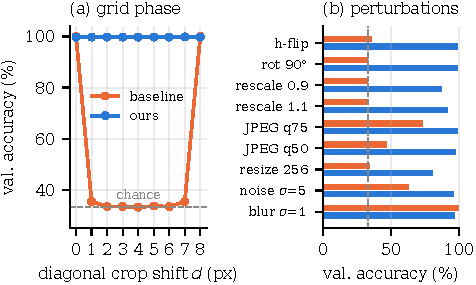
\includegraphics[width=\linewidth]{fig/probes.pdf}
  \caption{\textbf{What changed.} Held-out accuracy of the baseline (orange) and our model (blue). (a) Cropping a $504^2$ window whose origin is shifted by $(d,d)$: the baseline survives only $d\in\{0,8\}$, our model is flat at 99.7\%. (b) Post-processing applied before inference. Dashed: chance.}
  \label{fig:probes}
\end{figure}

\subsection{What does our model read differently?}
\Cref{fig:probes} perturbs the held-out images without retraining.
\emph{Lattice phase.} The baseline drops to chance for every shift that is not a multiple of 8 and for flips and rotations. These move or mirror the lattice without removing it, which confirms the diagnosis. Our model is unaffected (99.7\%).
\emph{Scale.} A $\pm10\%$ rescale is fatal for the baseline (33\%) and costs our model 8--12 points, although such factors occur in training. Halving the resolution, outside the training range, leaves our model at 80.9\%.
\emph{Compression and noise.} JPEG q50 costs our model 2 points (baseline: 53), and Gaussian noise with $\sigma{=}5$ costs it 3.5 points (baseline: 36). The one cost of robustness is blur: $\sigma{=}1$ costs our model 2.3 points and the baseline 0.1.

\begin{figure}[t]
  \centering
  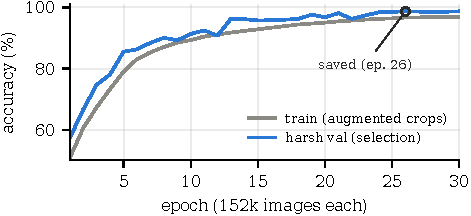
\includegraphics[width=\linewidth]{fig/curves_v4.pdf}
  \caption{\textbf{Training of our model.} Training accuracy on augmented crops and held-out accuracy under the harsh augmentation (used for selection).}
  \label{fig:curves}
\end{figure}

\subsection{Ablations and training behaviour}
\noindent\textbf{Crop size and class rebalancing.} A variant trained with $128^2$ crops and 20 copies of the smoothest 25\% of real images ties our model (dev 96.0\%). Its best-dev checkpoint (97.3\%, epoch 20) predicts 744 test images as real, so on 900 dev images a 1-point gain is noise. We therefore select on harsh validation.

\noindent\textbf{Invariance is slow to learn.} The baseline passes 99.9\% after two epochs of 12k images. Our model needs 21 epochs of 152k crops to pass 98\% on harsh validation (\cref{fig:curves}): invariance must be learnt from many shifted and rescaled examples. The held-out curves track training accuracy, so 30 epochs do not overfit.

\subsection{Error analysis}
\begin{figure}[t]
  \centering
  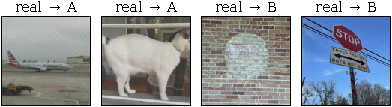
\includegraphics[width=\linewidth]{fig/failures.pdf}
  \caption{\textbf{Most confident errors of our model on dev}: real photographs labelled as Model~A or~B with probability ${>}0.99$. Each scene is ordinary and textured; none shows visible processing.}
  \label{fig:failures}
\end{figure}
The dev confusion matrix of our model (rows: true real/A/B) is
$\left[\begin{smallmatrix}268&10&22\\2&298&0\\1&0&299\end{smallmatrix}\right]$.
32 of its 35 errors are real images called fake. A and B are never confused with each other, and fake recall is 99.5\%. Real recall rises with texture, from 84\% for the smoothest quarter of real images to 92--93\% for the two most textured. Yet the most confident errors (\cref{fig:failures}) are ordinary textured photographs, which suggests our model partly relies on scene statistics of the training reals. On test, our model predicts 36 more real images than exist, so some fakes, plausibly those weakened by re-encoding, are called real. Either way, the errors are real versus fake, not A versus B.

\section{Conclusion}
\label{sec:conclusion}
A from-scratch artifact detector can be perfect on its own distribution and still fail completely after light post-processing, because it reads the generators' period-8 pattern at a fixed position. The fix needed no extra parameters and no test-time tricks. BlurPool down-sampling, crop training and broad offline augmentation give a single 11.17M-parameter model, applied once to the test image as given, that scores 95.3\% on test. The remaining error is not about processing but about content: real photographs of unfamiliar scenes, smooth ones more often, are labelled as fakes. Smaller crops and oversampling smooth real images did not change this. A consistency loss between clean and processed views of the same image, which ties the decision to the artifact rather than to the scene, is the clearest next step.

{
    \small
    \bibliographystyle{ieeenat_fullname}
    \bibliography{main}
}
\end{document}
